\documentclass{article}
% packages
\usepackage{amsmath,amssymb}
\usepackage{graphicx}
\usepackage{hyperref}

% directory of figures
%\graphicspath{ {figs} }

% latin bold lower
\newcommand{\ba}{\mathbf{a}}
\newcommand{\bc}{\mathbf{c}}
\newcommand{\be}{\mathbf{e}}
\newcommand{\bh}{\mathbf{h}}
\newcommand{\bp}{\mathbf{p}}
\newcommand{\bt}{\mathbf{t}}
\newcommand{\bs}{\mathbf{s}}
\newcommand{\bu}{\mathbf{u}}
\newcommand{\bv}{\mathbf{v}}
\newcommand{\bw}{\mathbf{w}}
\newcommand{\bx}{\mathbf{x}}
\newcommand{\by}{\mathbf{y}}
\newcommand{\bz}{\mathbf{z}}
\newcommand{\bm}{\mathbf{m}}

% latin bold upper
\newcommand{\bA}{\mathbf{A}}
\newcommand{\bB}{\mathbf{B}}
\newcommand{\bC}{\mathbf{C}}
\newcommand{\bI}{\mathbf{I}}
\newcommand{\bJ}{\mathbf{J}}
\newcommand{\bL}{\mathbf{L}}
\newcommand{\bM}{\mathbf{M}}
\newcommand{\bP}{\mathbf{P}}
\newcommand{\bQ}{\mathbf{Q}}
\newcommand{\bR}{\mathbf{R}}
\newcommand{\bT}{\mathbf{T}}
\newcommand{\bU}{\mathbf{U}}
\newcommand{\bV}{\mathbf{V}}
\newcommand{\bW}{\mathbf{W}}
\newcommand{\bX}{\mathbf{X}}
\newcommand{\bY}{\mathbf{Y}}
\newcommand{\bZ}{\mathbf{Z}}

% latin cal upper
\newcommand{\cF}{\mathcal{F}}
\newcommand{\cG}{\mathcal{G}}
\newcommand{\cI}{\mathcal{I}}
\newcommand{\cL}{\mathcal{L}}
\newcommand{\cM}{\mathcal{M}}
\newcommand{\cN}{\mathcal{N}}
\newcommand{\cS}{\mathcal{S}}
\newcommand{\cT}{\mathcal{T}}
\newcommand{\cW}{\mathcal{W}}
\newcommand{\cX}{\mathcal{X}}
\newcommand{\cZ}{\mathcal{Z}}

% latin bb upper
\newcommand{\bbE}{\mathbb{E}}
\newcommand{\bbI}{\mathbb{I}}
\newcommand{\bbP}{\mathbb{P}}
\newcommand{\bbR}{\mathbb{R}}
\newcommand{\bbX}{\mathbb{X}}
\newcommand{\bbY}{\mathbb{Y}}
\newcommand{\bbW}{\mathbb{W}}

% greek bold lower
\newcommand{\bepsilon}{\boldsymbol{\epsilon}}
\newcommand{\btheta}{\boldsymbol{\theta}}
\newcommand{\blambda}{\boldsymbol{\lambda}}
\newcommand{\bpi}{\boldsymbol{\pi}}
\newcommand{\bmu}{\boldsymbol{\mu}}
\newcommand{\bsigma}{\boldsymbol{\sigma}}
\newcommand{\bphi}{\boldsymbol{\phi}}

% greek bold upper
\newcommand{\bSigma}{\boldsymbol{\Sigma}}

\DeclareMathOperator*{\argmin}{arg\,min}
\DeclareMathOperator*{\argmax}{arg\,max}

% transpose
\newcommand{\T}{^{\text{\tiny\sffamily\upshape\mdseries T}}}


% if you need to pass options to natbib, use, e.g.:
\PassOptionsToPackage{numbers, sort, compress}{natbib}
% before loading neurips_2025


% ready for submission
%\usepackage{neurips_2025}


% to compile a preprint version, e.g., for submission to arXiv, add add the [preprint] option:
\usepackage[preprint]{neurips_2025}


% to compile a camera-ready version, add the [final] option, e.g.:
%\usepackage[final]{neurips_2024}


% to avoid loading the natbib package, add option nonatbib:
%\usepackage[nonatbib]{neurips_2024}


\usepackage[utf8]{inputenc} % allow utf-8 input
\usepackage[T1]{fontenc}    % use 8-bit T1 fonts
\usepackage{hyperref}       % hyperlinks
\usepackage{url}            % simple URL typesetting
\usepackage{booktabs}       % professional-quality tables
\usepackage{amsfonts}       % blackboard math symbols
\usepackage{nicefrac}       % compact symbols for 1/2, etc.
\usepackage{microtype}      % microtypography
\usepackage{xcolor}         % colors

%%%

\usepackage{subcaption}
\usepackage{graphicx}
\usepackage{multirow}
\usepackage{amsmath,amssymb,amsfonts}
\usepackage{amsthm}
\usepackage{mathrsfs}
\usepackage{xcolor}
\usepackage{textcomp}
\usepackage{manyfoot}
\usepackage{booktabs}
\usepackage{algorithm}
\usepackage{algorithmicx}
\usepackage{algpseudocode}
\usepackage{listings}

\newtheorem{theorem}{Theorem} % continuous numbers
%%\newtheorem{theorem}{Theorem}[section] % sectionwise numbers
%% optional argument [theorem] produces theorem numbering sequence instead of independent numbers for Proposition
\newtheorem{proposition}[theorem]{Proposition}% 
\newtheorem{lemma}{Lemma}% 
%%\newtheorem{proposition}{Proposition} % to get separate numbers for theorem and proposition etc.

\newtheorem{example}{Example}
\newtheorem{remark}{Remark}

\newtheorem{definition}{Definition}
\newtheorem{assumption}{Assumption}

%%%

\title{Neural Networks Loss Landscape Convergence in Hessian Low-Dimensional Space}


% The \author macro works with any number of authors. There are two commands
% used to separate the names and addresses of multiple authors: \And and \AND.
%
% Using \And between authors leaves it to LaTeX to determine where to break the
% lines. Using \AND forces a line break at that point. So, if LaTeX puts 3 of 4
% authors names on the first line, and the last on the second line, try using
% \AND instead of \And before the third author name.


\author{
  Tem Nikitin\\
  Moscow Institute of Physics and Technology\\
  Moscow, Russia\\
  \texttt{nikitin.artem.a@phystech.su}\\
  \And
  Nikita Kiselev\\
  Moscow Institute of Physics and Technology\\
  Moscow, Russia\\
  \texttt{kiselev.ns@phystech.su}\\
  \And
  Andrey Grabovoy\\
  Moscow Institute of Physics and Technology\\
  Moscow, Russia\\
  \texttt{grabovoy.av@phystech.su}\\
  \And
  Vladislav Meshkov\\
  Moscow Institute of Physics and Technology\\
  Moscow, Russia\\
  \texttt{meshkov.ns@phystech.su}\\
}


\begin{document}

\maketitle


\begin{abstract}
  Understanding how a neural network’s loss landscape changes as we add more training data is important for efficient training.
  Although larger datasets are known to reshape this high-dimensional surface, the point when extra data stop making a big difference
  is still unclear.

  In this paper, we study this issue and show that the loss landscape near a local minimum stabilizes once the dataset exceeds a
  certain size. To analyze this, we project the full parameter space onto a smaller subspace formed by the Hessian’s top eigenvectors.
  This low-dimensional view highlights how the loss surface changes in its most important directions. We then apply Monte Carlo sampling
  within this subspace to estimate these changes more precisely.

  We test our approach on standard image‑classification tasks and find that our low-dimensional analysis pinpoints when the landscape
  stops evolving. These findings clarify how dataset size affects optimization and offer practical guidance for balancing training cost
  with performance gains.
\end{abstract}


\textbf{Keywords:}
Neural networks, Loss landscape, Low-dimensional subspace, Hessian eigenvectors, Monte Carlo estimation, Dataset size threshold.


\section{Introduction}\label{sec:intro}

Neural networks are now essential in many areas --- image classification, language modeling, recommender systems, and more. As models and
datasets grow, we often see better accuracy and new breakthroughs. But bigger networks and data also demand more computation time and
resources, which can become prohibitive. While prior work has compared various optimization methods under fixed data and model sizes
\cite{soydaner2020comparison}, the question of when adding more training samples stops yielding significant gains remains largely
unanswered.

In this paper, we investigate exactly that: how the loss landscape changes as we increase the dataset size, and at what point further
data have little effect. Knowing this “minimum viable dataset size” --- a threshold beyond which new samples bring negligible
improvement --- can save both training time and data‑collection effort. We also relate this threshold to generalization behavior, along
the lines of \cite{wu2017towards}.

To study this, we use the Hessian of the loss function as a proxy for local curvature. Computing the full Hessian is expensive, so we
project the parameter space onto a low‑dimensional subspace formed by its top eigenvectors. Our main contributions are:

\begin{enumerate}
  \item Constructing a Hessian‑based projection that captures the principal curvature directions.
  \item Applying Monte Carlo and other sampling methods to identify when the loss landscape stabilizes as dataset size grows.
  \item Visualizing the projected loss surface around local minima to illustrate these changes.
  \item Deriving theoretical criteria --- using results from The Matrix Cookbook \cite{petersen2012matrix} --- to predict when additional
        samples have minimal impact.
\end{enumerate}

This approach is novel in linking low‑rank Hessian estimation to a concrete dataset threshold, enabling more cost‑effective data
collection and a clearer understanding of how data scale interacts with loss geometry. We validate our method on MNIST
\cite{deng2012mnist} and Fashion‑MNIST \cite{xiao2017fashion}, demonstrating how to balance computational cost against accuracy gains.

\textbf{Organization.} The rest of the paper is structured as follows. Section~2 reviews related work. Section~3 introduces notation
and preliminaries. Section~4 derives theoretical bounds on Hessian spectra and the loss‐difference norm. Section~5 presents our
empirical studies. We discuss the implications in Section~6 and conclude in Section~7. Additional experiments and proofs are
provided in Appendix~A.


\section{Related Work}\label{sec:rw}

\textbf{Hessian-based Analysis.}
The loss landscape of neural networks has been extensively studied using Hessian-based techniques, which illuminate convergence
behavior and curvature properties \cite{kiselev2024unraveling}. Empirical work shows that near local minima the Hessian often has low
effective rank, indicating a small "active subspace" spanned by a few large eigenvalues \cite{sagun2018empirical}. Ghorbani et al.
\cite{ghorbani2019investigation} examined how these large eigenvalues emerge during training and shape optimization dynamics.
Meshkov et al. \cite{meshkov2024convnets} extended this analysis to fully connected and convolutional architectures, though broader
validation across architectures remains an open challenge.

\textbf{Loss Landscape Geometry and Dataset Size.}
Another research direction explores how dataset size influences model performance and landscape geometry. Networks trained on larger
datasets tend to find flatter, wider minima that generalize better \cite{wu2017towards}. Yet, acquiring and processing massive data is
costly, motivating studies of optimal data–model trade‑offs \cite{hoffmann2022training}. Li et al. \cite{li2018visualizing} developed
visualization tools that reveal how dataset size, initialization, and architecture affect the topology of loss surfaces.

\textbf{Algorithmic Stability and Landscape Sensitivity.}
Algorithmic stability, which measures how small changes in the training set affect the learned model, provides theoretical bounds on
generalization error \cite{bousquet2002stability}. Elisseeff et al. \cite{elisseeff2005stability} extended stability analysis to
randomized algorithms such as bagging and ensemble methods, deriving non-asymptotic generalization guarantees. In our context,
stability theory underpins the intuition that, beyond a certain dataset size, further samples cause negligible changes to the loss
curvature. Our Monte Carlo–based Hessian projection method directly leverages this perspective, using top eigenvectors to quantify
and visualize when the loss landscape stabilizes as new data are added.


\section{Preliminaries}\label{sec:prelim}

\subsection{General notation}

We consider a $S$-class classification problem. Let $\bx \in \bX$ be an input and $y \in \mathcal Y = \{1, \dots, S\}$ its label. A
neural network with parameters $\bw \in \bOmega \subset \mathbb R^P$ defines a mapping $f_{\bw} : \bX \to \mathbb R^S$. Given a dataset
$$
  \mathcal D =
  \{(\bx_i, y_i)\}_{i=1}^N
$$
of $m$ i.i.d. samples, and a per-sample loss $\ell \bigl( f_{\bw}(\bx_i), y_i \bigr)$ (e.g. cross–entropy), we define
$$
  \ell_i(\bw) =
  \ell \bigl( f_{\bw}(\bx_i) , y_i \bigr)\,.
$$

\begin{definition}
  The empirical loss on the first $k$ samples is
  $$
    \cL_k(\bw) =
    \frac1k \sum_{i=1}^k \ell_i(\bw),
  $$
  so that the full-sample loss is $\cL(\bw) = \cL_N(\bw)$.
\end{definition}

A simple telescoping gives the difference
$$
  \cL_{k+1}(\bw) - \cL_k(\bw) =
  \frac{\ell_{k+1}(\bw) - \cL_k(\bw)}{k+1}\,.
$$

\begin{definition}
  The Hessian of $\cL_k$ at $\bw$ is
  $$
    \bH_k(\bw) =
    \nabla^2_{\bw} \cL_k(\bw) =
    \frac1k \sum_{i=1}^k \nabla^2_{\bw} \ell_i(\bw),
  $$
  and, similarly, the full-sample Hessian is $\bH(\bw) = \bH_N(\bw) = \nabla^2_{\bw} \cL_N(\bw)$.
\end{definition}

To capture the overall change in the landscape when adding one more sample, we introduce a $\Delta$‑function:

\begin{definition}
  Let $p(\bw)$ be a weighting (e.g. peaked near a local minimum). Define
  $$
    \Delta_k =
    \int \bigl( \cL_{k+1}(\bw) - \cL_k(\bw) \bigr)^2\, p(\bw)\, d\bw.
  $$
\end{definition}

We study the behavior of $\Delta_k$ as $k \to \infty$ and define a threshold:

\begin{definition}
  Fix a tolerance $\Delta > 0$. The \emph{sufficient sample size} is
  $$
    K =
    \inf \{ k \mid \forall\, k' \ge k : \; \Delta_{k'} < \Delta\}.
  $$
  When $k \ge K$, adding further samples changes the loss landscape by less than $\Delta$.
\end{definition}

\subsection{Assumptions}

We make the following standard assumptions to simplify our analysis around a local minimizer~$\bw^*$.

\begin{assumption}
  The point $\bw^*$ is a common local minimizer for both $\cL_k$ and $\cL_{k+1}$, i.e.
  $$
    \nabla \cL_k(\bw^*) =
    \nabla \cL_{k+1}(\bw^*) =
    0.
  $$
\end{assumption}

Under this assumption, a second‑order Taylor expansion of $\cL_k$ about $\bw^*$ gives
$$
  \cL_k(\bw) \approx
  \cL_k(\bw^*) + \tfrac12\, (\bw - \bw^*)^{\T} \bH_k(\bw^*)\, (\bw - \bw^*).
$$

\begin{assumption}
  At the minimizer $\bw^*$, the loss values for consecutive sample sizes are the same:
  $$
    \cL_{k+1}(\bw^*) =
    \cL_k(\bw^*).
  $$
\end{assumption}

\begin{assumption}
  The parameters $\bw$ are distributed according to a density $p(\bw)$ (e.g. a Gaussian prior centered at $\bw^*$).  Then
  $$
    \Delta_k =
    \int \bigl(\cL_{k+1}(\bw)-\cL_k(\bw)\bigr)^2\, p(\bw)\, d\bw =
    \mathbb{E} \left( \cL_{k+1}(\bw) - \cL_{k}(\bw) \right)^2 =
  $$
  $$
    \mathbb D \bigl[ \cL_{k+1}(\bw) - \cL_k(\bw) \bigr] +
    \Bigl( \mathbb E \bigl[ \cL_{k+1}(\bw) - \cL_k(\bw) \bigr] \Bigr)^2.
  $$
\end{assumption}


\section{Method: Projection onto Dominant Eigen-Directions and Loss Landscape Approximation}

Working with the full Hessian $\mathbf{H}_k(\bw)$ of a neural network is computationally expensive due to the high dimensionality
of the parameter space $\bOmega$. To reduce this cost, we project the parameters onto a lower‑dimensional subspace spanned by the
$d$ dominant eigenvectors of the Hessian at a local minimum $\bw^*$.

The justification for this projection is that, empirically, the Hessian has low effective rank near a minima \cite{sagun2018empirical}:
only a few eigenvalues are significantly above zero, while the rest are negligible.  Therefore, directions corresponding to small
eigenvalues contribute little to loss variation.  Retaining only the top $d$ eigenvectors yields a compact yet informative representation
of the most important curvature directions.

For illustration, Figure~\ref{fig:evgen} plots the top few eigenvalues of $\bH(\bw^*)$ in descending order. We compute these dominant
eigenvalues using the iterative power‐method described at \cite{hessian-eigenthings}.

\begin{figure}[!htbp]
  \centering
  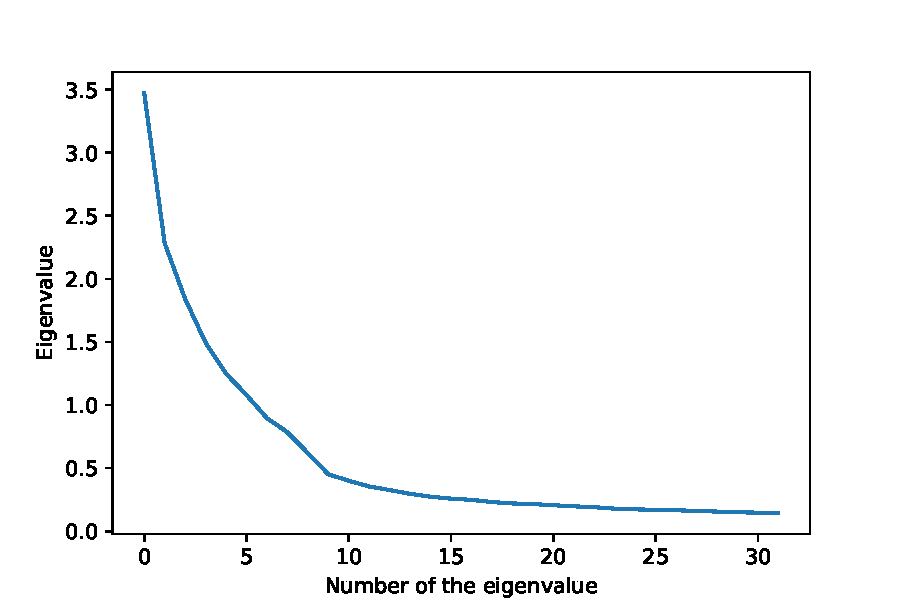
\includegraphics[width=0.7\textwidth]{img/eigenvalues.pdf}
  \caption{Top eigenvalues of $\bH(\bw^*)$ in descending order.}
  \label{fig:evgen}
\end{figure}

Concretely, let
$$
  \bP =
  \bigl[ \mathbf{e}_1, \dots, \mathbf{e}_d \bigr]
$$
be the matrix whose columns are the top $d$ eigenvectors.  We write any parameter vector as
$$
  \bw =
  \bw^* + \bP\, \btheta, \quad
  \btheta \in \mathbb R^d.
$$
Substituting into a second‑order Taylor expansion of $\cL_k$ around $\bw^*$ gives
$$
  \cL_k\bigl(\bw^* + \bP\,\btheta\bigr) \approx
  \cL_k(\bw^*) + \tfrac12\, \btheta^{\T}\! \bigl( \bP^{\T}\, \bH_k(\bw^*)\, \bP\bigr)\, \btheta =
  \cL_k(\bw^*) + \tfrac12\, \btheta^{\T} \bLambda_k\, \btheta,
$$
where
$$
  \bLambda_k =
  \bP^{\T}\, \bH_k(\bw^*)\, \bP =
  \operatorname{diag} \bigl( \lambda_k^{(1)}, \dots, \lambda_k^{(d)} \bigr).
$$
An identical expansion holds for $\cL_{k+1}$, yielding $\bLambda_{k+1}$ from the Hessian on $k+1$ samples.

\begin{theorem}[Approximate $\Delta_k$ via Eigenvalues]
  Under the assumption that $\btheta \sim \mathcal N(0, \sigma^2 \mathbf I_d)$, the change in loss can be estimated by
  $$
    \Delta_k =
    \mathbb E \bigl[ \cL_{k+1}(\bw) - \cL_k(\bw) \bigr]^2 \approx
    \frac{\sigma^4}{4}\, \Biggl( 2 \sum_{i=1}^d (\lambda_{k+1}^{(i)} - \lambda_k^{(i)})^2
    + \Bigl( \sum_{i=1}^d (\lambda_{k+1}^{(i)} - \lambda_k^{(i)}) \Bigr)^2 \Biggr).
  $$
\end{theorem}

\begin{remark}
  Assuming $\mathbb{E}(\btheta) = \mathbf{0}$ is natural when centering the sampling distribution at the minimum.
\end{remark}

This formula uses only the top $d$ eigenvalues, so it is efficient to compute even for very large models.
In practice, it provides an upper bound on the empirical $\Delta_k$ and thus a reliable criterion for determining when the
dataset size is sufficient.


\section{Experiments}

To validate our theoretical estimates, we perform a set of experiments that track how the loss landscape changes as we grow the
training set.

\paragraph{Datasets.}
We evaluate on MNIST \cite{deng2012mnist} and Fashion‑MNIST \cite{xiao2017fashion}, each containing 60,000 training and 10,000 test
grayscale images of size $28\times28$ pixels.

\paragraph{Model Architecture.}
All experiments use a simple multilayer perceptron (MLP) with ReLU activations.  We keep the same architecture—number of hidden layers
and hidden units—across all runs to ensure a fair comparison.

\paragraph{Experimental Procedure.}
\begin{enumerate}
  \item \textbf{Random‐direction visualization:} As an initial sanity check, we project the parameters onto two random directions and
        plot the resulting 3D loss landscapes and their squared differences.
  \item \textbf{Hessian‐based analysis:} We then repeat the visualization and compute $\Delta_k$ by projecting onto the top two
        (and up to $d = 10$) eigenvectors of the Hessian.  This directly tests our eigenvalue‐based approximation and the convergence behavior
        predicted by theory.
\end{enumerate}

All code and detailed configuration files are available in our GitHub repository.

\subsection{Preliminary Experiment: Projection onto Random Directions}
\subsubsection{Visualizing the Loss Landscape}

To build intuition for how the loss surface changes with training‐set size, we first project the model parameters onto two random
directions. Specifically, we pick two random vectors $\mathbf v_1, \mathbf v_2 \in \mathbb R^P$ in parameter space and study the
subspace they span.

We then evaluate the empirical loss
$$
  \cL_k(\bw) =
  \frac1k \sum_{i=1}^k \ell_i(\bw),
$$
where $\ell_i(\bw) = \ell (f_\bw(\bx_i), y_i)$, over a grid in the $(\alpha, \beta)$ plane defined by
$$
  \bw(\alpha,\beta) =
  \bw^* + \alpha\, \mathbf v_1 + \beta\, \mathbf v_2, \quad
  (\alpha, \beta) \in [-1,1]^2.
$$

\begin{enumerate}
  \item \textbf{Grid Sampling.}
        We form a uniform grid of $(\alpha, \beta)$ pairs in $[-1,1]\times[-1,1]$ with a fixed step size.
  \item \textbf{Loss Computation.}
        For each $(\alpha,\beta)$, we set $\bw=\bw(\alpha,\beta)$, keep the base weights $\bw^*$ fixed, and compute both
        $\cL_k(\bw)$ and $\cL_{k+1}(\bw)$.
  \item \textbf{Aggregated Metrics.}
        \begin{itemize}
          \item The surface $\cL_k(\alpha,\beta)$ visualizes how the mean loss changes over the grid.
          \item The surface $\bigl( \cL_{k+1} (\alpha, \beta) - \cL_k (\alpha, \beta) \bigr)^2$ highlights where adding one sample
                causes the largest change.
        \end{itemize}
  \item \textbf{3D Visualization.}
        We render two side‐by‐side 3D plots:
        \begin{itemize}
          \item \emph{Left:} $\cL_k (\alpha, \beta)$ vs. $(\alpha, \beta)$.
          \item \emph{Right:} $\bigl( \cL_{k+1} (\alpha, \beta) - \cL_k (\alpha, \beta) \bigr)^2$ vs. $(\alpha, \beta)$.
        \end{itemize}
\end{enumerate}

\begin{figure}[!htbp]
  \hspace*{-2.2cm}
  \subfloat{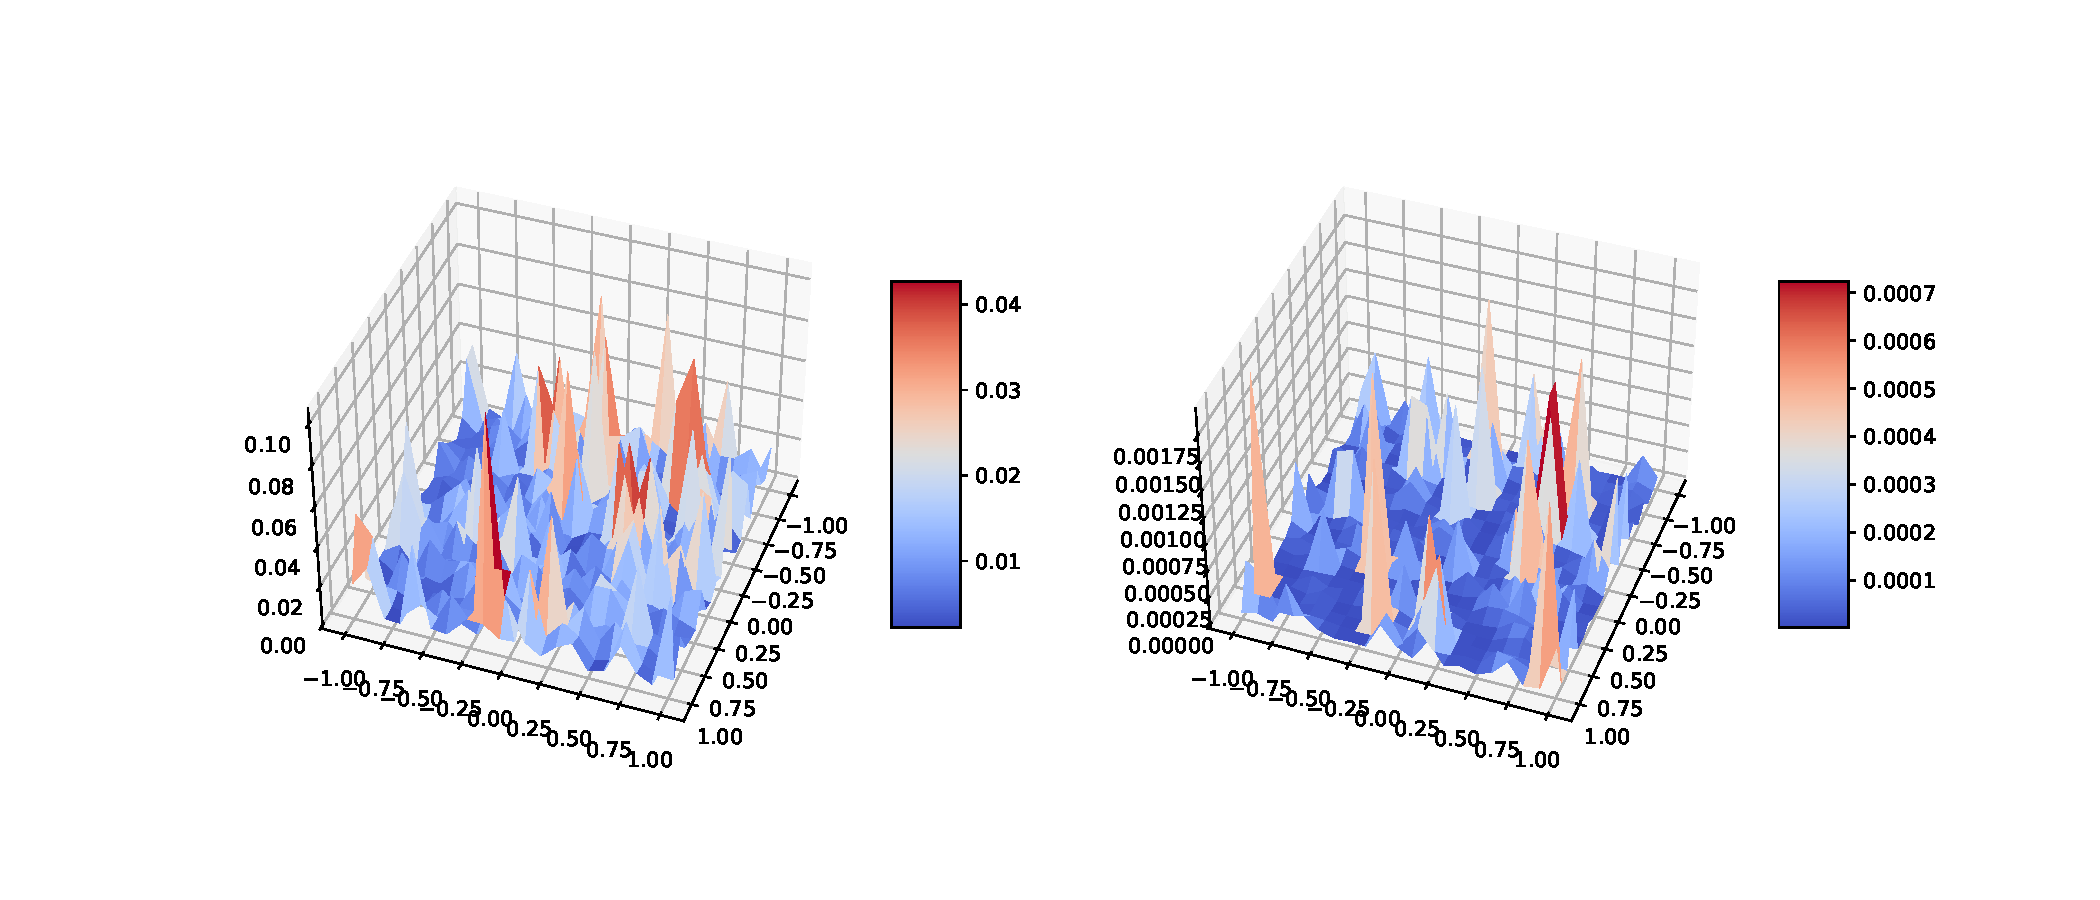
\includegraphics[width=1.3\textwidth]{img/loss_random_1_2.pdf}}
  \caption{$\cL_k$ (left) and $\bigl[ \cL_{k+1}(\btheta) - \cL_k(\btheta) \bigr]^2$ (right) for small $k$, projected onto the two random vectors.}
  \label{fig:loss_random_small}
\end{figure}

\begin{figure}[!htbp]
  \hspace*{-2.2cm}
  \subfloat{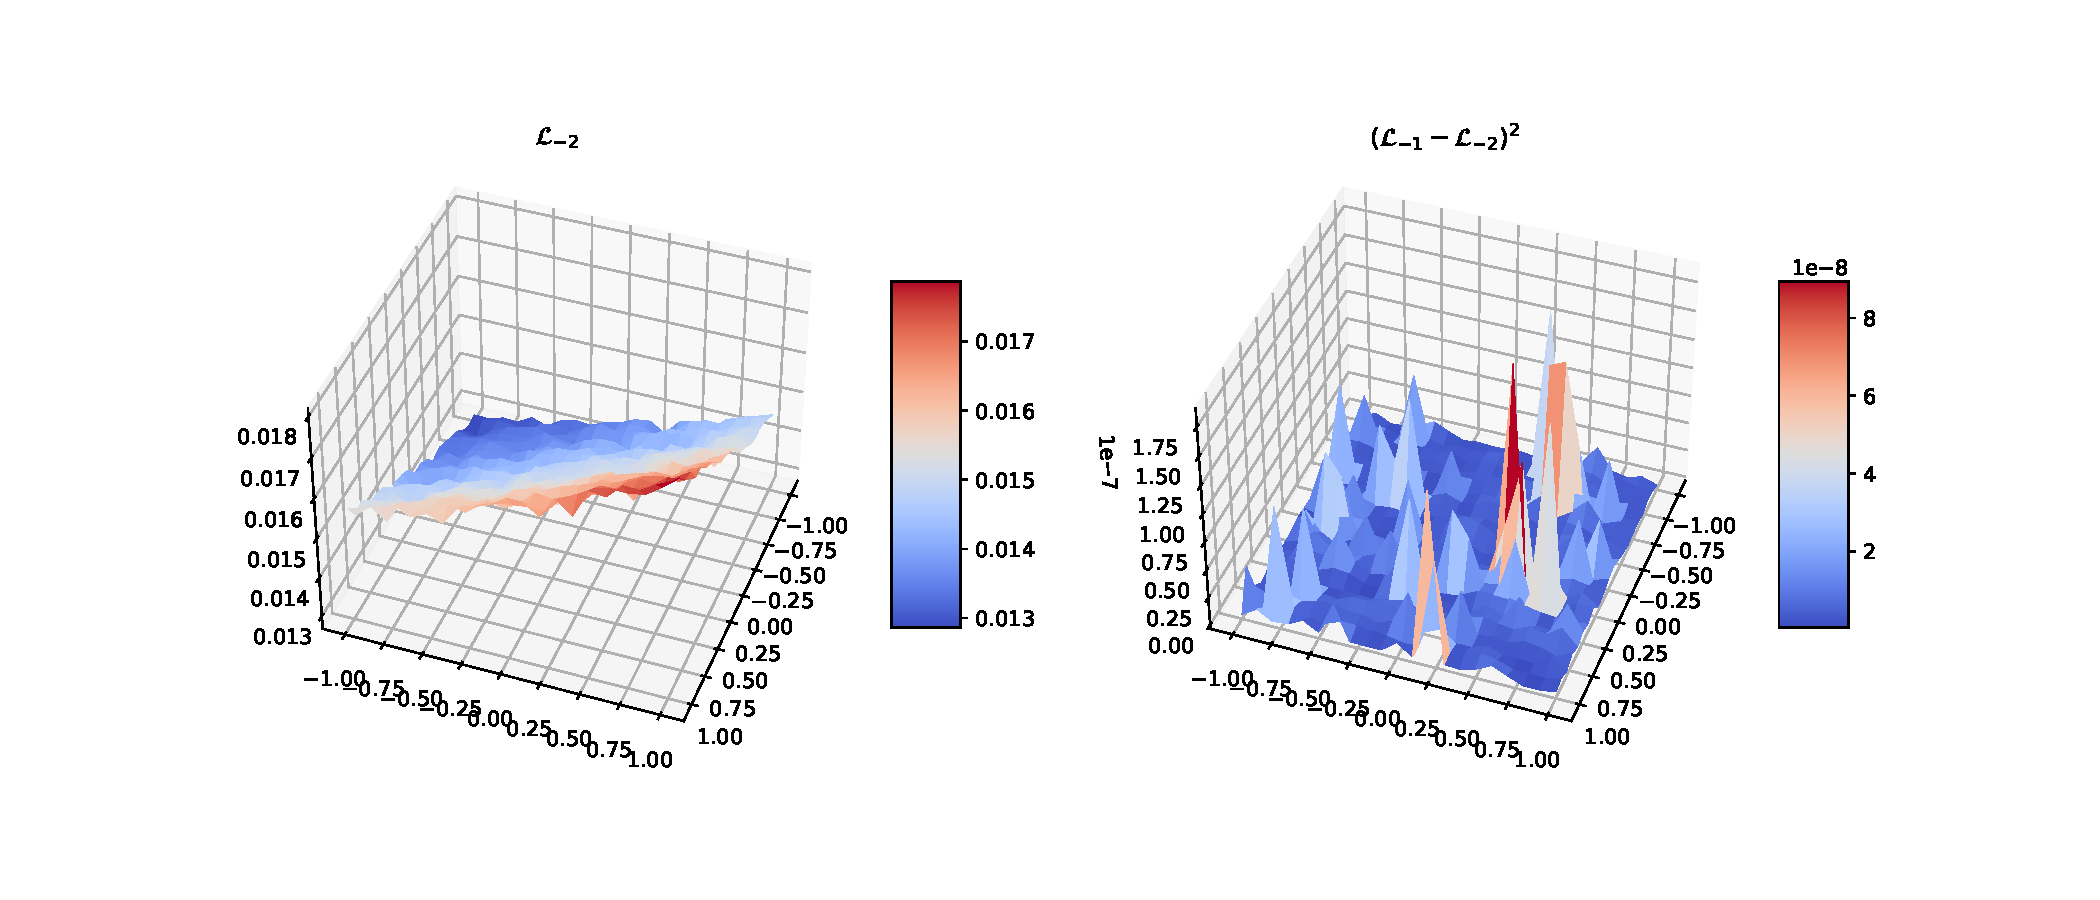
\includegraphics[width=1.3\textwidth]{img/loss_random_-2_-1.pdf}}
  \caption{$\cL_k$ (left) and $\bigl[ \cL_{k+1}(\btheta) - \cL_k(\btheta) \bigr]^2$ (right) for maximum $k$, projected onto the two random vectors.}
  \label{fig:loss_random_big}
\end{figure}

\paragraph{Loss Landscape for the Small Dataset}
In Figure~\ref{fig:loss_random_small}, the loss surface is highly irregular, with sharp peaks and deep valleys.
This irregularity indicates that with very few training samples, the model is extremely sensitive to small parameter perturbations.
The squared difference surface also exhibits large spikes, confirming that adding a single data point can cause substantial local changes
in the loss.

\paragraph{Loss Landscape for the Full Dataset}
In contrast, Figure~\ref{fig:loss_random_big} shows a much smoother loss surface with gentle slopes. The overall loss
values are lower --- reflecting the averaging effect of more samples --- and the squared difference surface is correspondingly much smaller.
This smoothing demonstrates that as the dataset grows, the local optimum stabilizes, and additional samples produce only minor
adjustments to the loss landscape. Hence, beyond a certain dataset size, further data have negligible impact on the shape of the loss
surface.

\subsubsection{Visualizing the \texorpdfstring{$\Delta_k$}{Delta k} Function}

To study how the loss landscape converges as the dataset grows, we estimate and plot the function
$$
  \Delta_k =
  \mathbb{E} \bigl[ \cL_{k+1}(\bw) - \cL_k(\bw) \bigr]^2
$$
via a Monte Carlo approximation using Gaussian perturbations in parameter space. The steps are:

\begin{enumerate}
  \item \textbf{Sample directions.}
        Starting from a fixed trained model with parameters $\bw^*$, draw $T$ independent random vectors
        $$
          \btheta^{(t)} \sim \mathcal{N} (\mathbf 0, \sigma^2 \mathbf I_d), \quad
          t = 1, \dots, T.
        $$

  \item \textbf{Perturb parameters.}
        For each sample, form a perturbed parameter set
        $$
          \bw^{(t)} =
          \bw^* + \btheta^{(t)}.
        $$

  \item \textbf{Evaluate loss differences.}
        Compute
        $$
          \cL_k \bigl( \bw^{(t)} \bigr) \quad
          \text{and} \quad
          \cL_{k+1} \bigl( \bw^{(t)} \bigr),
        $$
        then calculate the squared difference
        $$
          d_t =
          \bigl[ \cL_{k+1} (\bw^{(t)}) - \cL_k (\bw^{(t)}) \bigr]^2.
        $$

  \item \textbf{Compute Monte Carlo estimate.}
        Approximate
        $$
          \Delta_k \approx
          \frac{1}{T} \sum_{t=1}^T d_t.
        $$
        Increasing $K$ reduces the variance of this estimator.

  \item \textbf{Plot results.}
        We plot $\Delta_k$ versus $k$ to observe its decay. We also plot the scaled quantity
        $$
          \Delta_k \cdot k^2
        $$
        alongside to highlight an $\mathcal O(1 / k)$ convergence rate.
\end{enumerate}

Figures~\ref{fig:delta_random_sigma} and \ref{fig:delta_random_dim} present the behavior of the function
$$
  \Delta_k =
  \mathbb{E} \bigl[ \cL_{k+1}(\bw) - \cL_k(\bw) \bigr]^2
$$
under different Monte Carlo sampling settings and projection subspace sizes. Each figure isolates one variable:

\begin{itemize}
  \item Figure~\ref{fig:delta_random_sigma}: varying the Gaussian variance $\sigma$.
  \item Figure~\ref{fig:delta_random_dim}: varying the subspace dimension $d$.
\end{itemize}

\begin{figure}[!htbp]
  \hspace*{-2.6cm}
  \subfloat{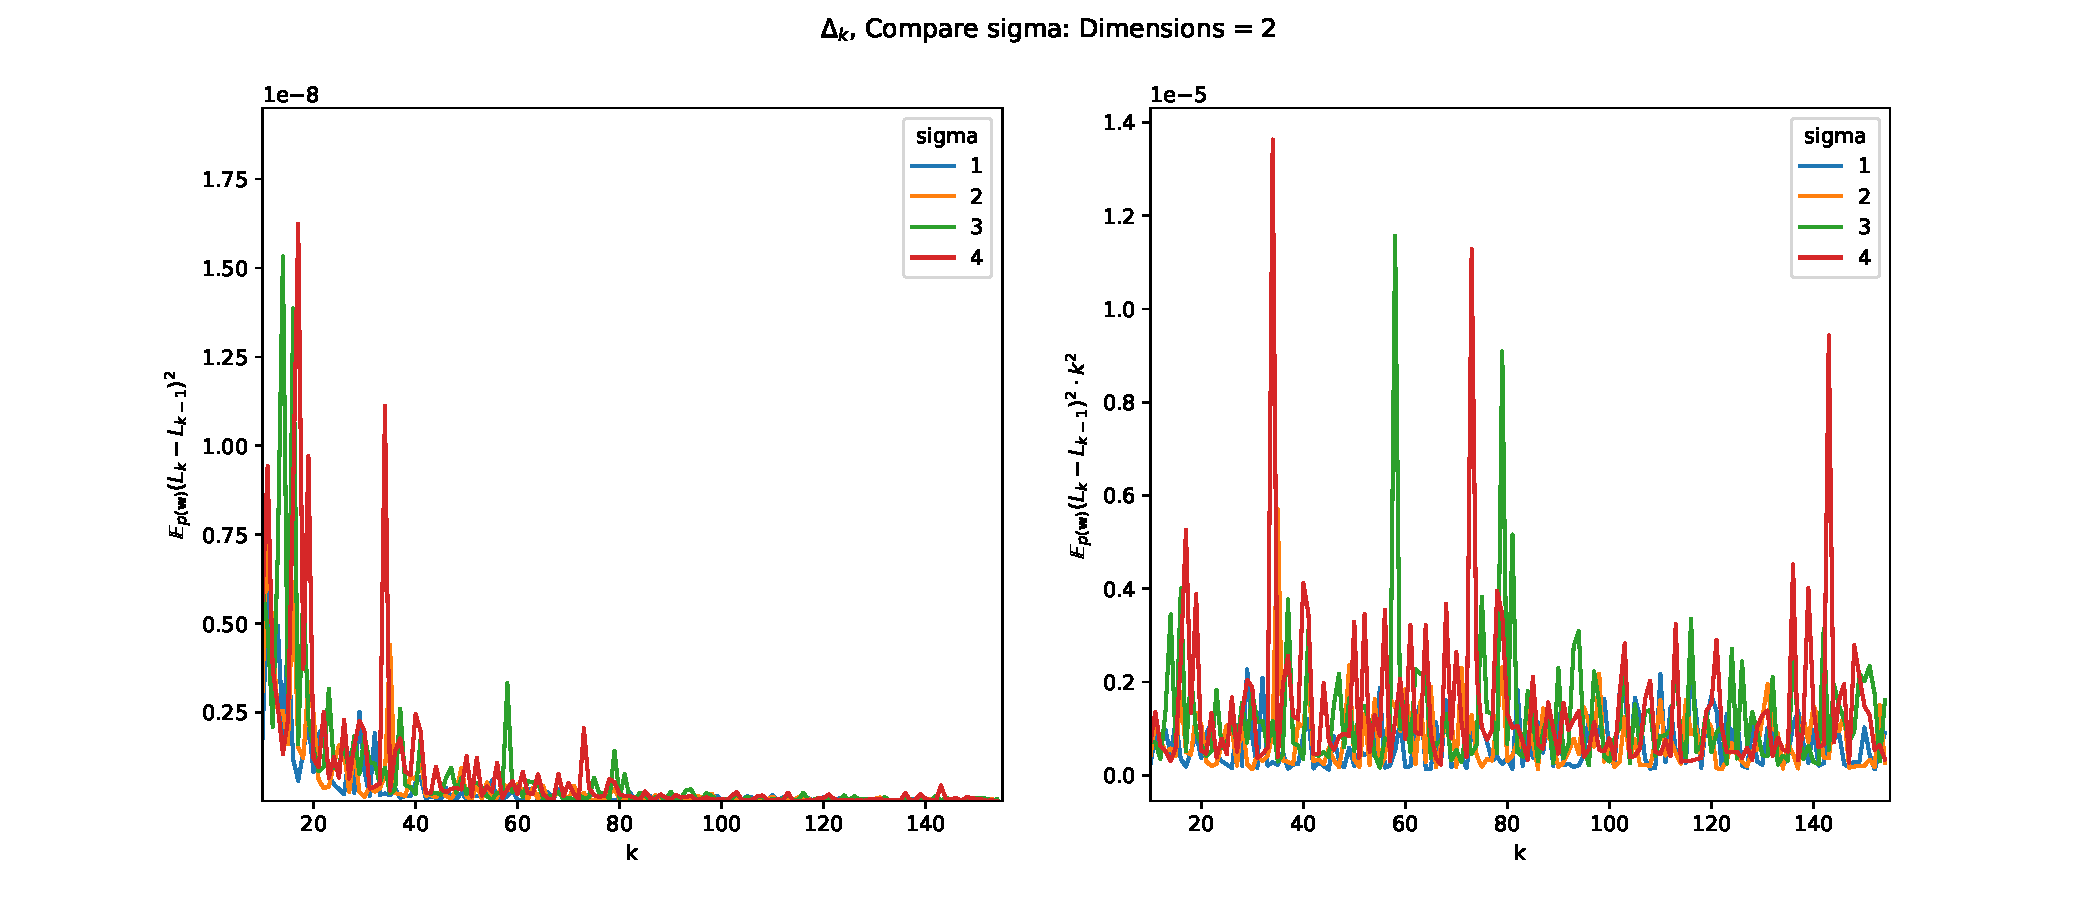
\includegraphics[width=1.35\textwidth]{img/delta_random_sigma_2_64.pdf}}
  \caption{$\Delta_k$ (left) and $\Delta_k \cdot k^2$ (right), varying the Gaussian variance with fixed $d = 2$.}
  \label{fig:delta_random_sigma}
\end{figure}

\begin{figure}[!htbp]
  \hspace*{-2.6cm}
  \subfloat{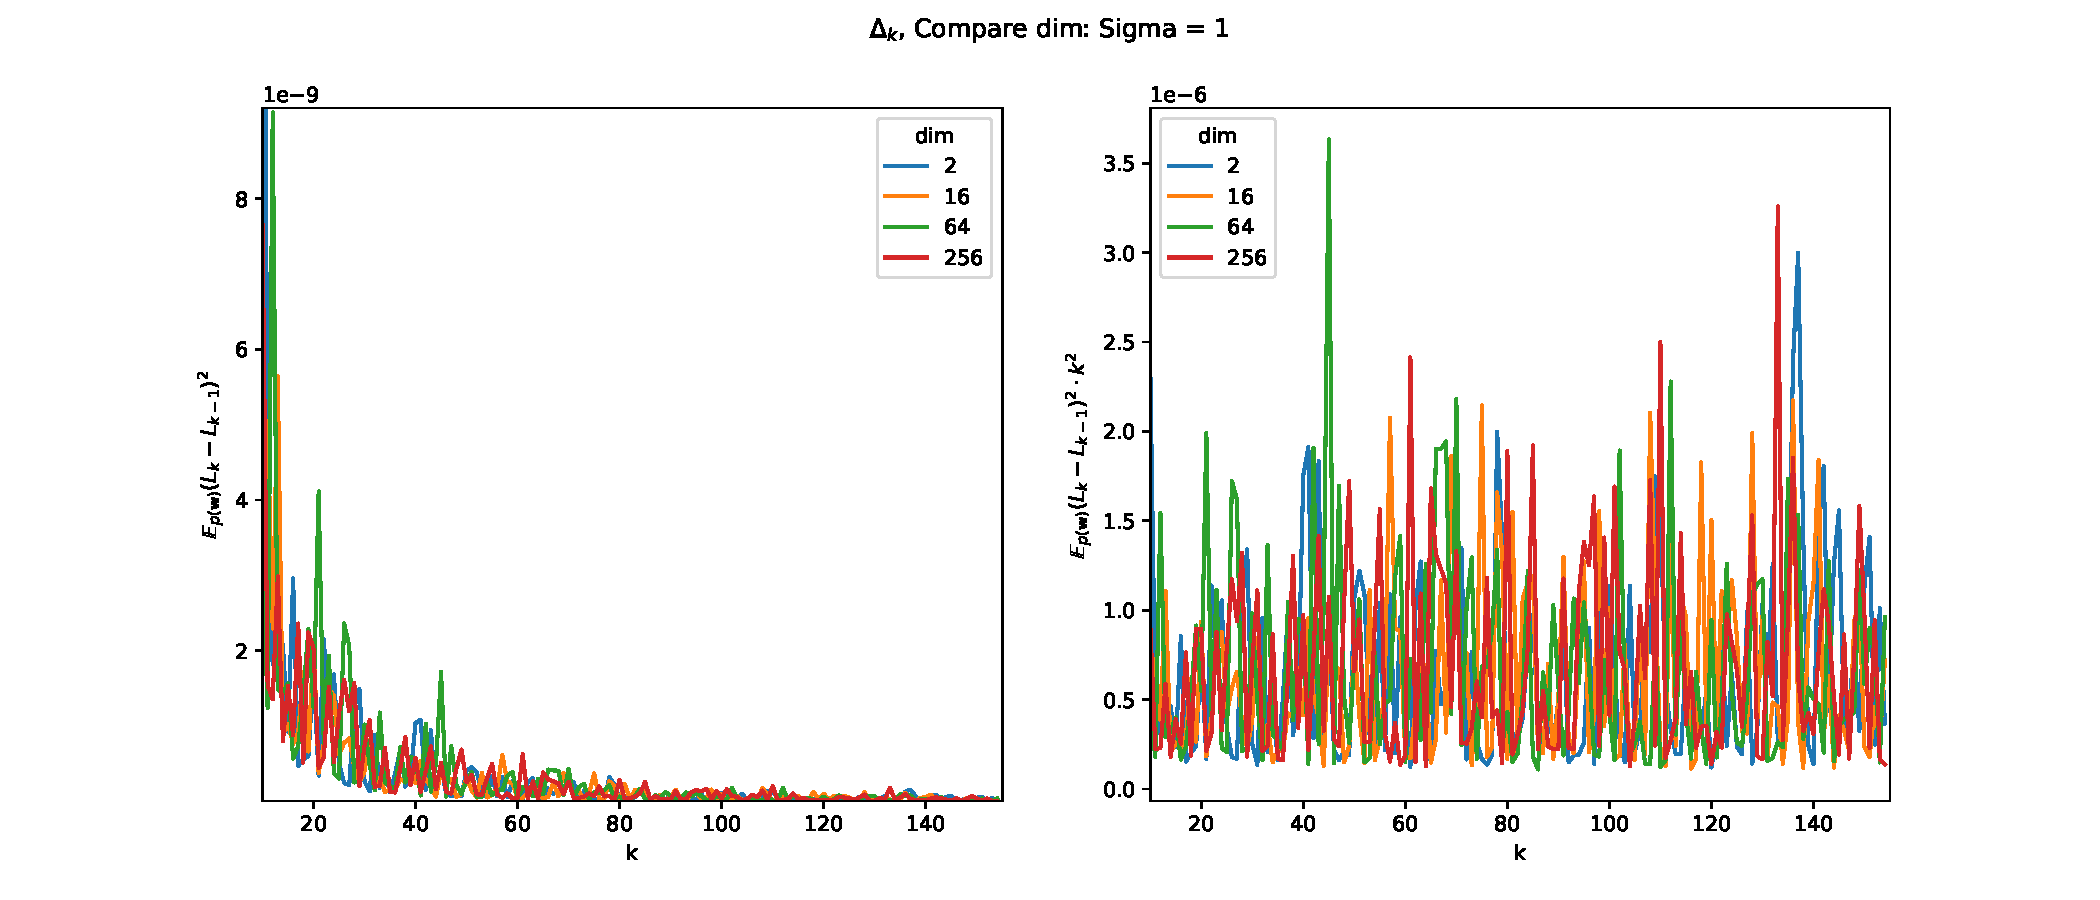
\includegraphics[width=1.35\textwidth]{img/delta_random_dim_1_64.pdf}}
  \caption{$\Delta_k$ (left) and $\Delta_k \cdot k^2$ (right), varying the subspace dimension with fixed $\sigma = 1$.}
  \label{fig:delta_random_dim}
\end{figure}

\paragraph{Comparing Different Variances \texorpdfstring{$\sigma$}{sigma}}
Figure~\ref{fig:delta_random_sigma} shows that varying the Gaussian variance $\sigma$ produces no substantial change in the shape or
magnitude of the $\Delta_k$ curves. This insensitivity likely stems from using random projection directions: since they do not align
with the dominant curvature axes of the Hessian, scaling those directions has little impact on the estimated loss differences.

\paragraph{Comparing Different Subspace Dimensions}
Figure~\ref{fig:delta_random_dim} shows that, when using random directions, increasing the projection dimension $d$ does not
significantly alter the overall shape of $\Delta_k$. This suggests that only a few directions dominate the variation --- motivating our
focus on Hessian‐based projections in the main experiment.

In all cases, the right‐hand plots (showing $\Delta_k \cdot k^2$) exhibit a roughly $\mathcal O(1 / k)$ decay, confirming that the
incremental effect of adding one more sample diminishes proportionally to $1 / k$ as the dataset grows.

The preliminary experiments show that the loss landscape indeed smooths out and becomes more stable as the training set size $N$
increases. However, because we used random projection directions, these results capture only a generic view of stability. This
observation motivates our main experiment, in which we project onto the Hessian’s top eigenvectors --- i.e., the directions of greatest
curvature --- to obtain a more precise understanding of when and how the loss surface converges.

\subsection{Moving Forward: Projection onto Dominant Hessian Eigenvectors}

\paragraph{Projection Directions.}
In the main experiment, we replace random directions with the $d$ eigenvectors of the Hessian at the local minimizer $\bw^*$ that
correspond to its largest eigenvalues.  Prior work \cite{sagun2018empirical} shows these top modes capture nearly all of the
non‑negligible curvature, and Figure~\ref{fig:evgen} confirms a rapid eigenvalue decay. Fixing $d=10$ balances computational cost and
fidelity, and our tests on Fashion‑MNIST and CIFAR demonstrate that this choice suffices even for complex architectures.

\paragraph{Objectives.}
By projecting onto these principal directions, we aim to:
\begin{itemize}
  \item Obtain a clearer view of how the loss surface changes as $k$ grows, since these directions drive the largest loss variations.
  \item Accurately identify the threshold $k^*$ at which further data cause only negligible shifts in the local curvature.
  \item Empirically validate our theoretical $\Delta_k$ estimates by comparing them against Monte Carlo measurements in this eigenvector
        subspace.
\end{itemize}

\subsubsection{Visualizing the Loss Landscape}

Figures~\ref{fig:loss_eigen_small} and \ref{fig:loss_eigen_big} display 3D plots of $\cL_k(\btheta)$ (left) and 
$\bigl[ \cL_{k+1}(\btheta) - \cL_k(\btheta) \bigr]^2$ (right), where $\btheta$ varies over the span of the top two Hessian eigenvectors.
 The procedure mirrors the random‑direction case but uses these maximally informative axes.

\begin{figure}[!htbp]
  \hspace*{-2.2cm}
  \subfloat{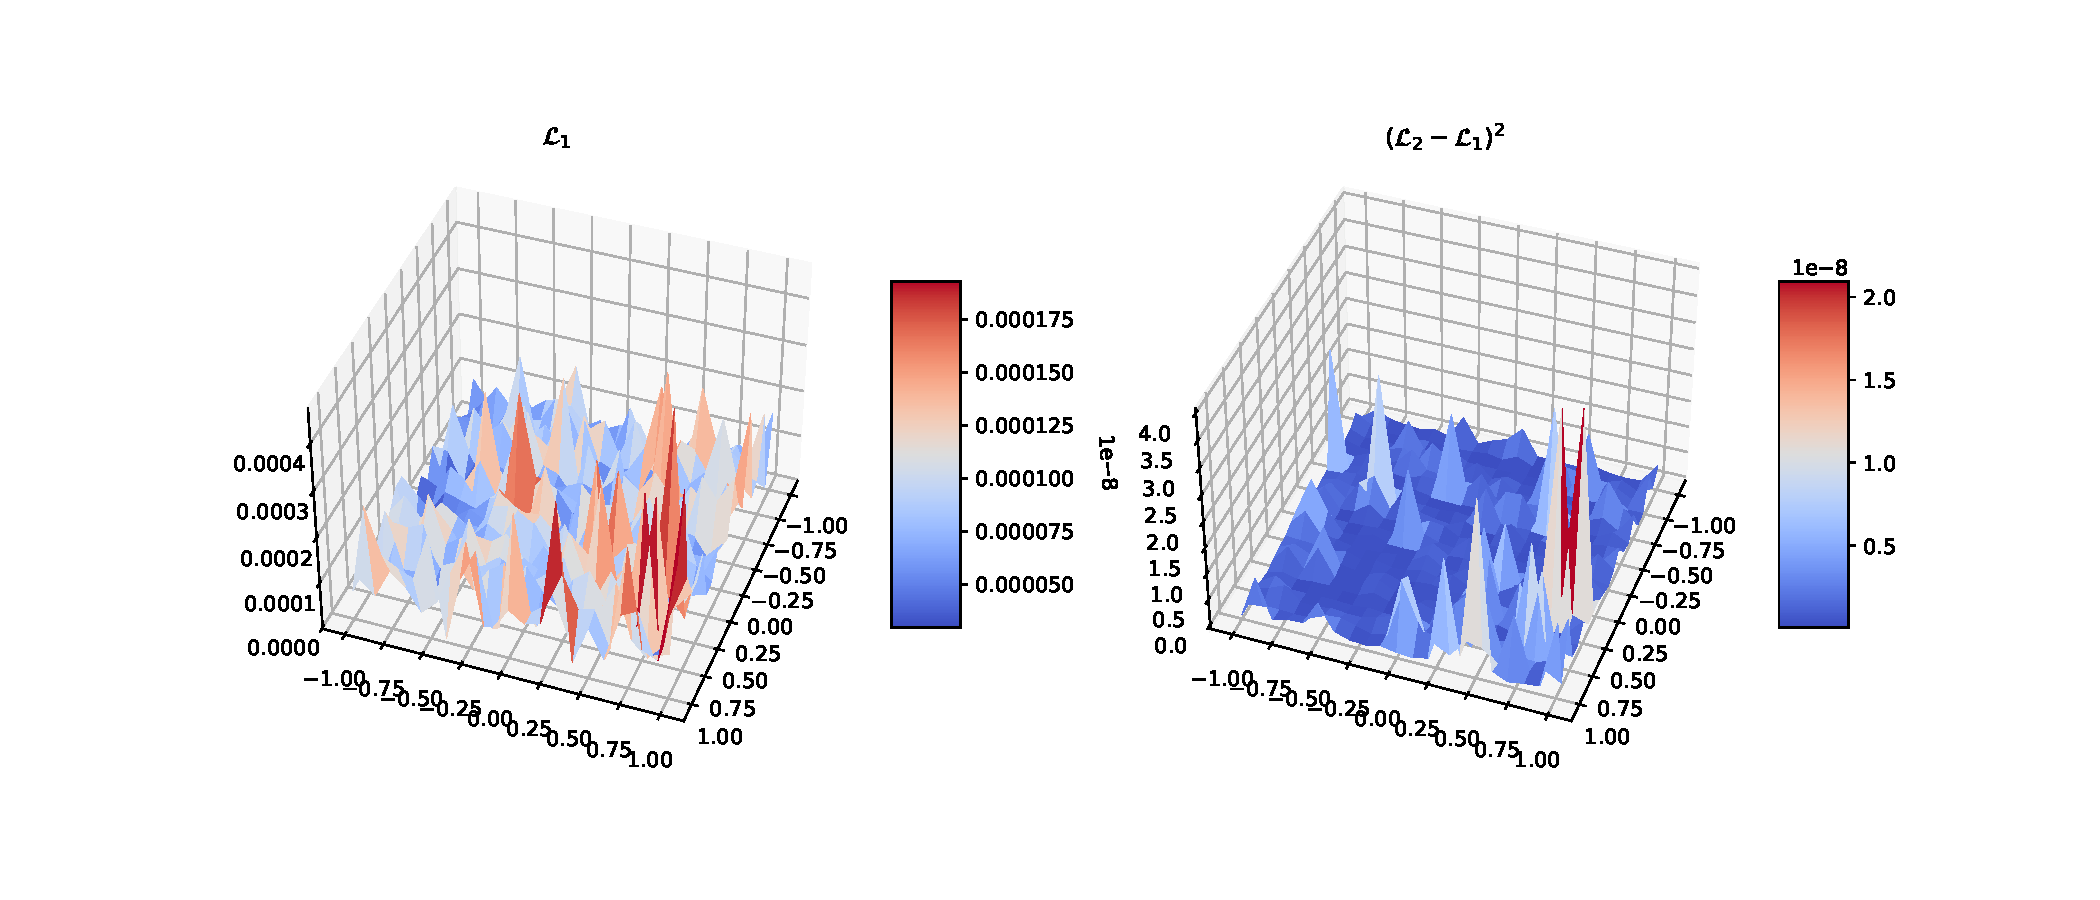
\includegraphics[width=1.3\textwidth]{img/loss_eigen_1_2.pdf}}
  \caption{$\cL_k$ (left) and $\bigl[ \cL_{k+1}(\btheta) - \cL_k(\btheta) \bigr]^2$ (right) for small $k$, projected onto the top two Hessian eigenvectors.}
  \label{fig:loss_eigen_small}
\end{figure}

\begin{figure}[!htbp]
  \hspace*{-2.2cm}
  \subfloat{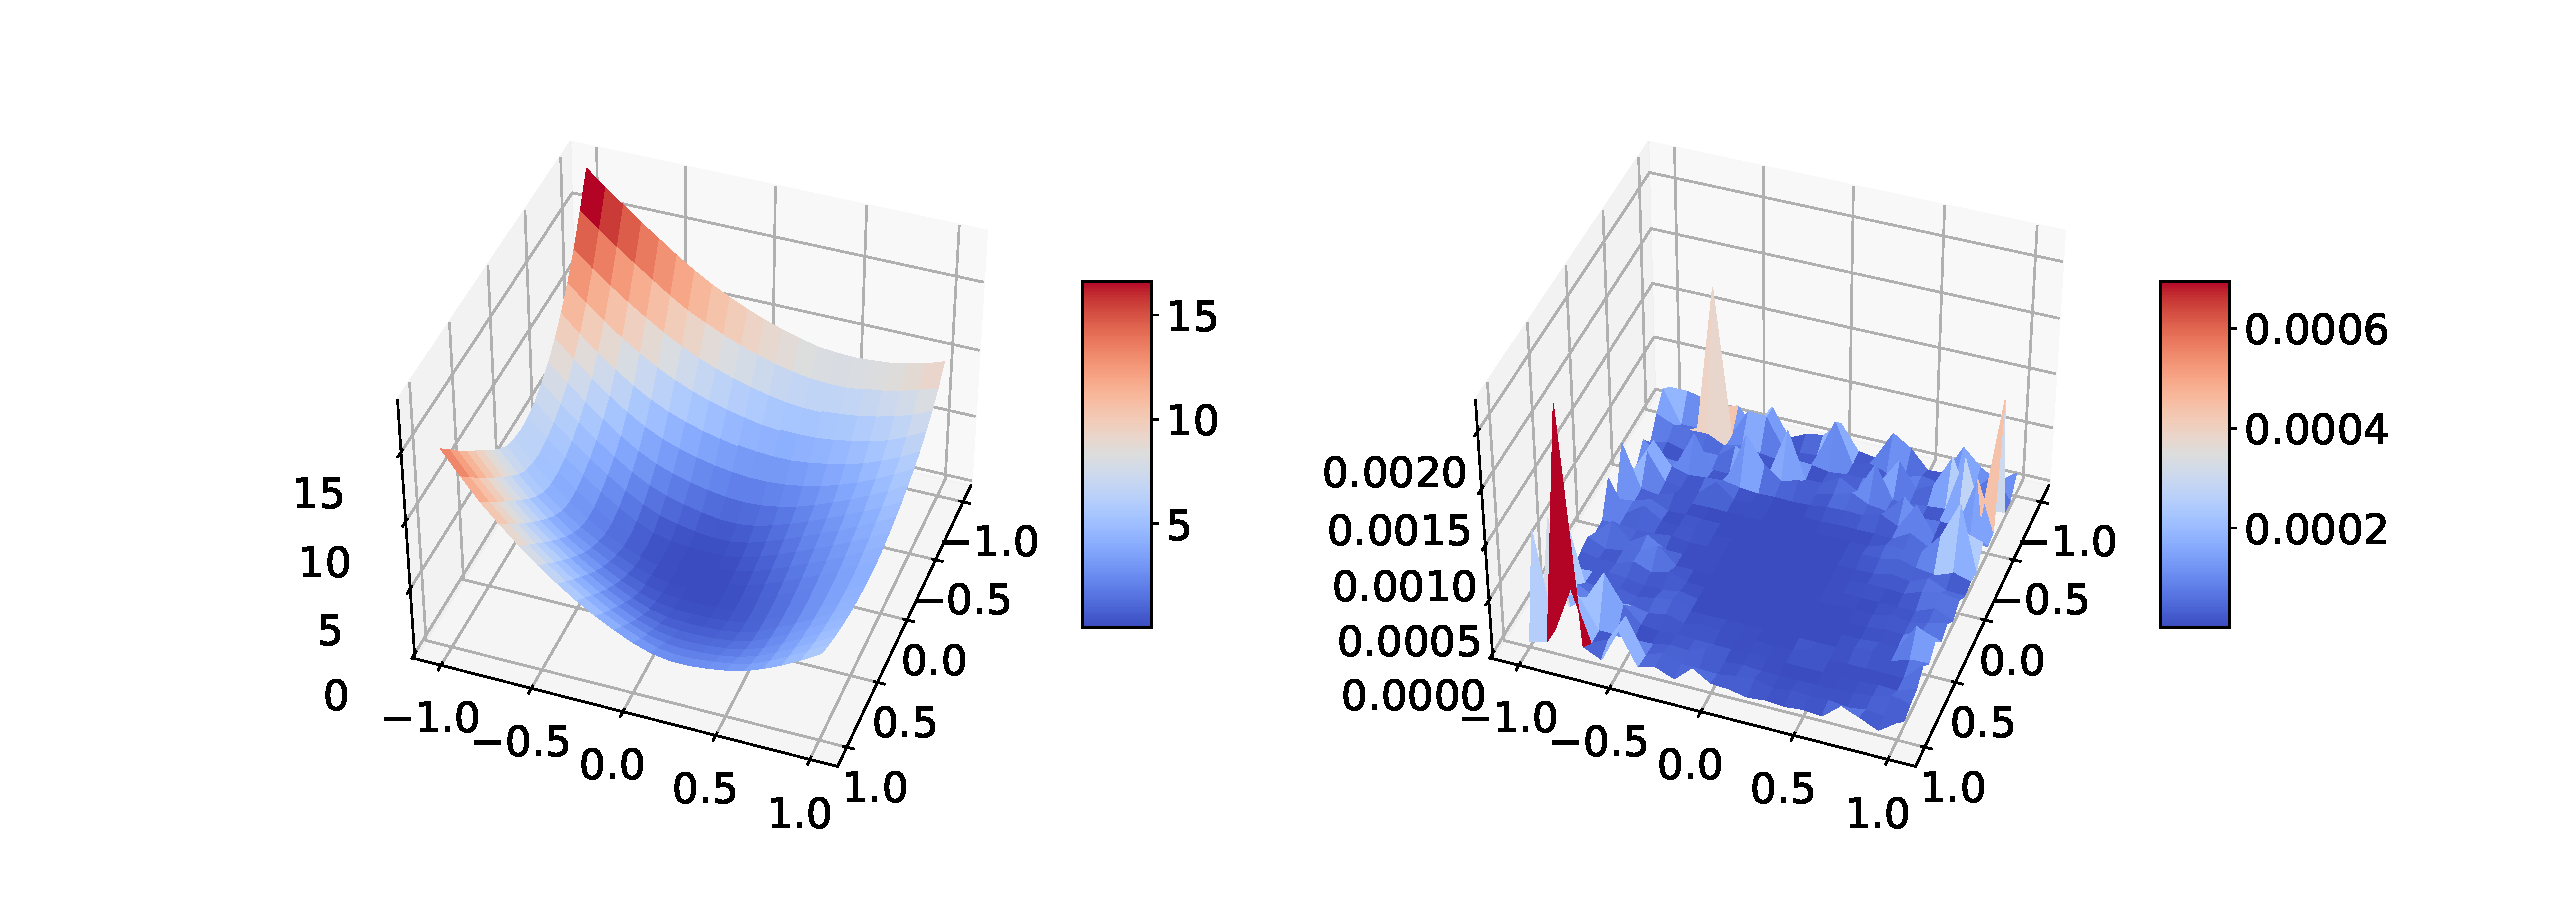
\includegraphics[width=1.3\textwidth]{img/loss_eigen_-2_-1.pdf}}
  \caption{$\cL_k$ (left) and $\bigl[ \cL_{k+1}(\btheta) - \cL_k(\btheta) \bigr]^2$ (right) for maximum $k$, projected onto the top two Hessian eigenvectors.}
  \label{fig:loss_eigen_big}
\end{figure}

\paragraph{Loss Landscape for the Small Dataset}
In Figure~\ref{fig:loss_eigen_small}, the loss surface projected onto the top two Hessian eigenvectors is
noticeably more structured and less erratic than in the random‐direction case. This confirms that these eigenvectors capture the
most influential directions of loss variation. The squared‐difference plot also shows larger peaks, indicating that the model is
highly sensitive to new data along these key axes when $k$ is small.

\paragraph{Loss Landscape for the Full Dataset}
By contrast, Figure~\ref{fig:loss_eigen_big} shows a much smoother loss surface and a greatly reduced squared‐difference.
As the dataset grows, the loss changes less along the principal curvature directions, and the model’s local behavior stabilizes.
Notably, even at large $k$, the squared difference remains higher than in the random‐direction experiment, providing a practical upper
bound on landscape fluctuations. These findings reinforce that projecting onto the top eigenvectors effectively reveals the convergence
behavior of the loss landscape and helps intuitively understand the existence of the point beyond which additional data have minimal impact.

\subsubsection{Visualizing the \texorpdfstring{$\Delta_k$}{Delta k} Function}

\begin{figure}[!htbp]
  \hspace*{-2.6cm}
  \subfloat{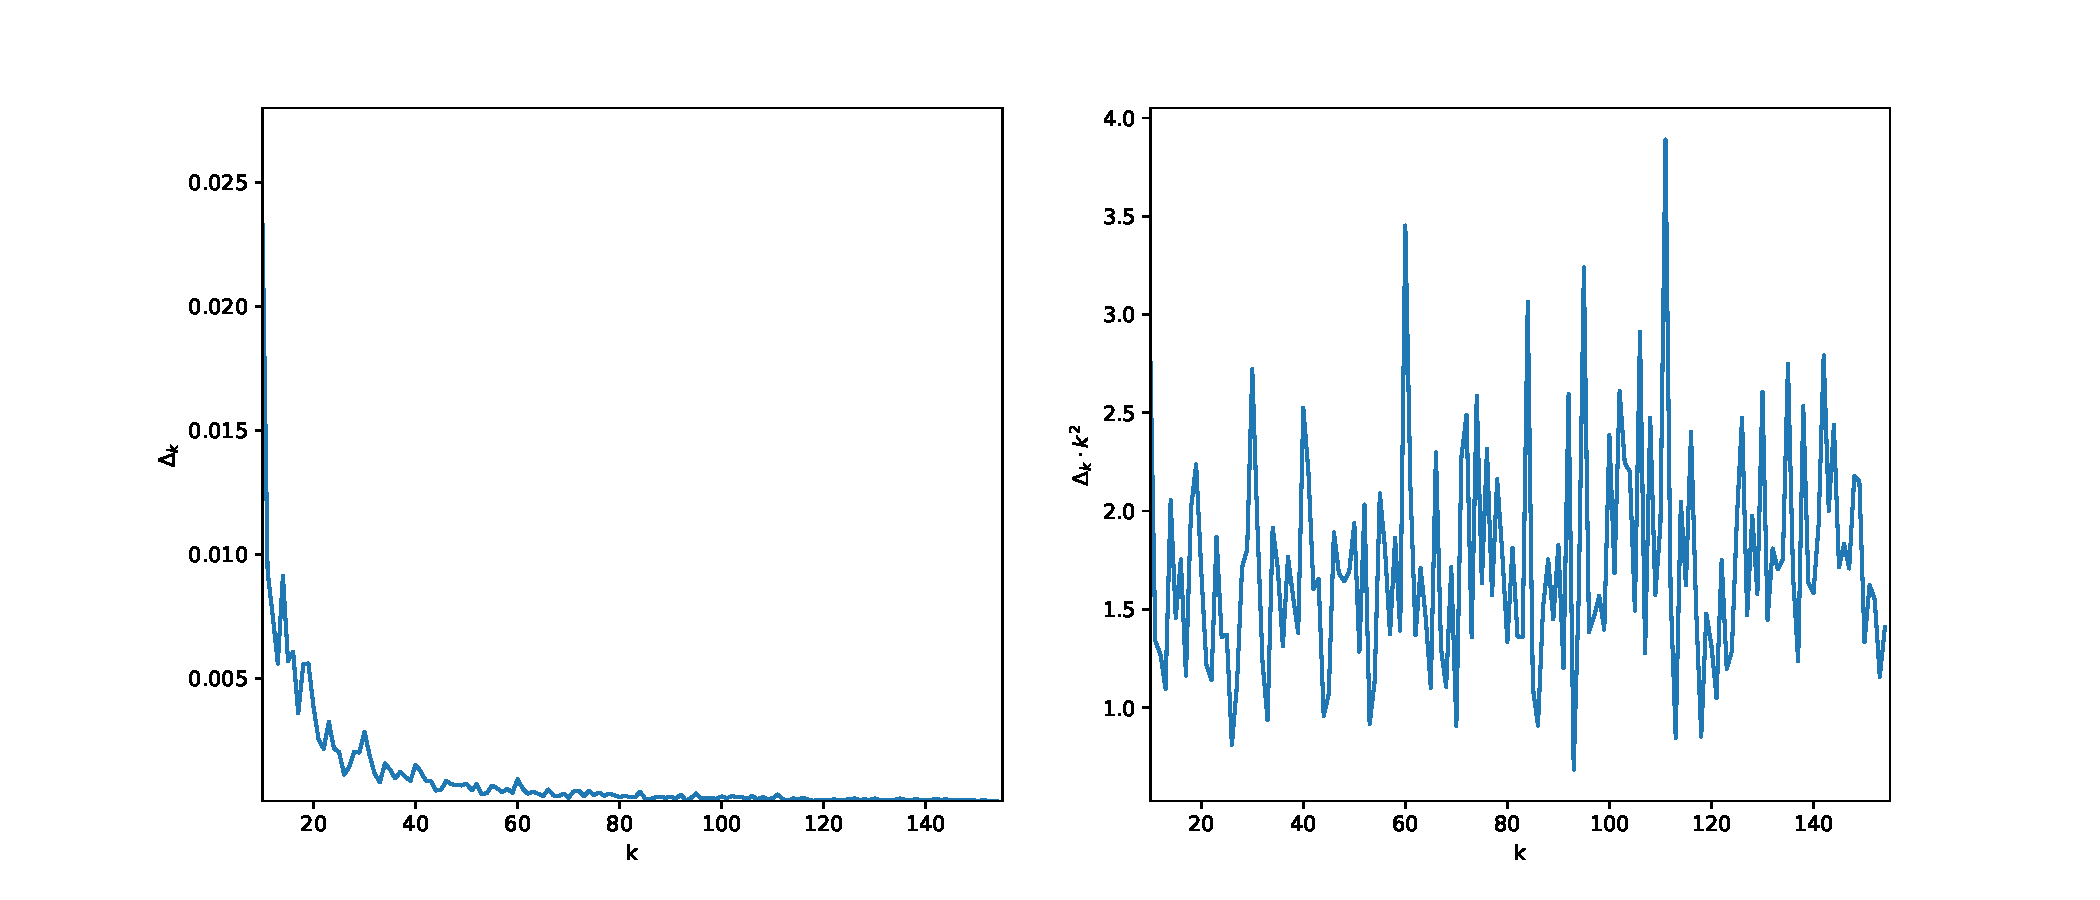
\includegraphics[width=1.35\textwidth]{img/delta_eigen_1_10_64.pdf}}
  \caption{$\Delta_k$ (left) and $\Delta_k \cdot k^2$ (right)}
  \label{fig:delta_eigen}
\end{figure}

Figure~\ref{fig:delta_eigen} presents the Monte Carlo estimate of $\Delta_k$ in the subspace spanned by the top $d = 10$
Hessian eigenvectors. Compared to the random‐direction experiment, $\Delta_k$ here has a higher value --- reflecting the
large curvature captured by these eigenvectors. The right‐hand plot of $\Delta_k\cdot k^2$
confirms an approximate $O(1 / k)$ convergence rate. These observations show that projecting onto the leading eigen-directions not only
highlights the greatest loss sensitivity but also yields a reliable upper bound on how quickly the landscape stabilizes as more data are
added.

\subsection{Main Experiment: Theoretical vs. Empirical \texorpdfstring{$\Delta_k$}{Delta k}}

In this experiment, we compare our Hessian‐based theoretical estimate of $\Delta_k$ with the empirical Monte Carlo measurements.

We approximate $\Delta_k$ by
$$
  \Delta_k \approx
  \frac{\sigma^4}{4}\, \Biggl( 2 \sum_{i=1}^d (\lambda_{k+1}^{(i)} - \lambda_k^{(i)})^2
  + \Bigl( \sum_{i=1}^d (\lambda_{k+1}^{(i)} - \lambda_k^{(i)}) \Bigr)^2 \Biggr).
$$
where $\{\lambda_k^{(i)}\}_{i=1}^d$ and $\{\lambda_{k+1}^{(i)}\}_{i=1}^d$ are the top $d$ Hessian eigenvalues at sample sizes $k$ and $k + 1$,
and $\sigma$ is the perturbation variance.

\begin{enumerate}
  \item \textbf{Model \& subspace size.} Train a network to obtain $\bw^*$. Choose $d$ based on the rapid eigenvalue decay in
        Figure~\ref{fig:evgen}.
  \item \textbf{Eigenvalue computation.} For each $k$ in the range of interest (typically the largest $K$ sizes), compute the top
        $d$ eigenvalues via the power method.
  \item \textbf{Theoretical $\Delta_k$.} Plug these eigenvalues into the formula above to obtain a sequence of theoretical estimates.
  \item \textbf{Empirical $\Delta_k$.} Independently estimate $\Delta_k$ by Monte Carlo sampling of perturbations along the same
        top‐$d$ eigenvectors as it was in the previous experiment.
  \item \textbf{Comparison.} Plot both theoretical and empirical $\Delta_k$ on the same axes to assess how tightly the theory bounds
        the observed values.
\end{enumerate}

\begin{figure}[!htbp]
  \subfloat{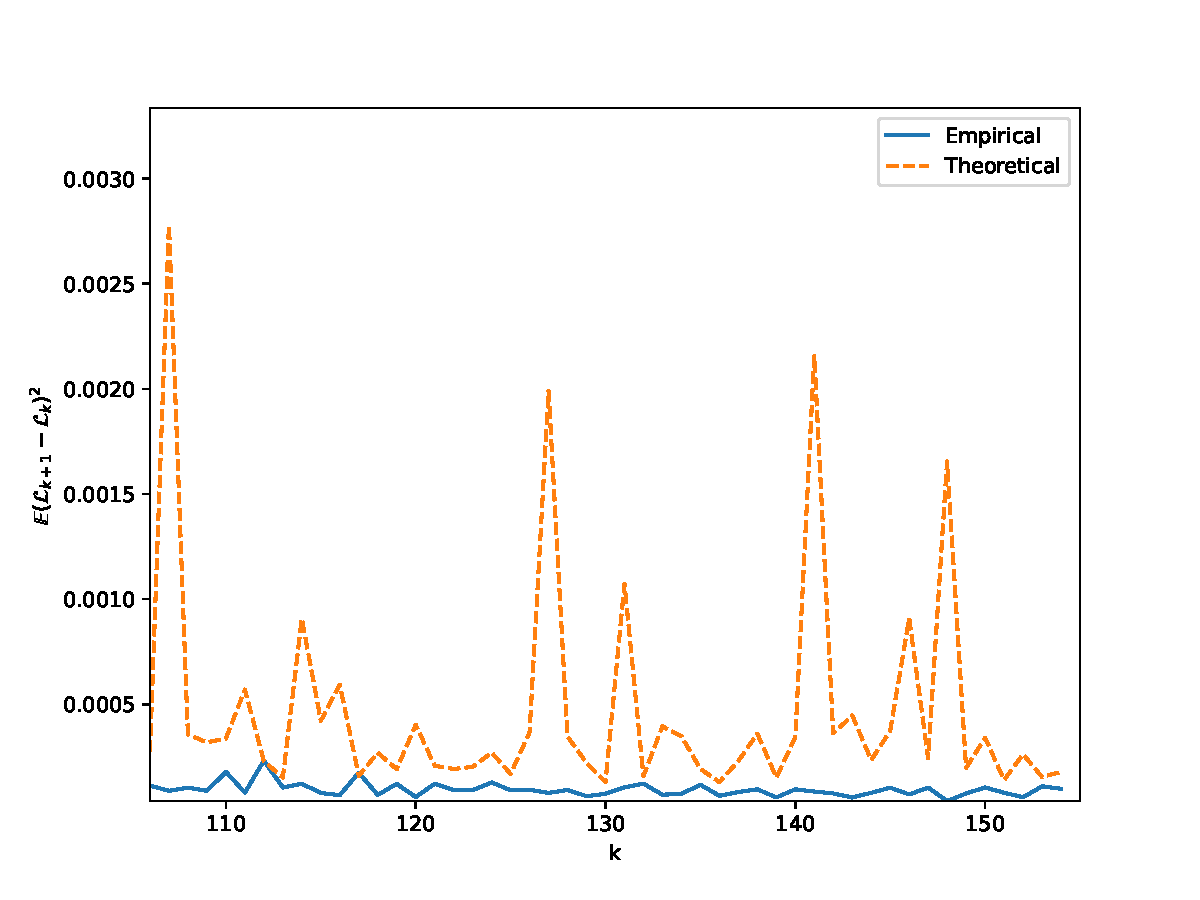
\includegraphics[width=1\textwidth]{img/delta_border_1_10_64.pdf}}
  \caption{Theoretical and Empirical $\Delta_k$}
  \label{fig:delta_eigen_comparison}
\end{figure}

Figure~\ref{fig:delta_eigen_comparison} shows the theoretical estimate of $\Delta_k$ (dashed line) alongside the empirical Monte Carlo
measurements (solid line).  Across all values of $k$, the theory curve remains above the empirical one, demonstrating that our
eigenvalue‐based formula provides a valid upper bound for the true loss‐landscape changes.


\section{Discussion}\label{sec:disc}

The gap between the theoretical and empirical curves arises because the estimate uses only the top $d$ eigenvalues.
Therefore, focusing on the leading modes yields a reliable and efficient criterion for determining when
adding more data has negligible effect on the local loss geometry.

Our Hessian‐projection framework provides a clear picture of how a neural network’s loss landscape evolves with training–set size.
By restricting attention to the $d$ principal curvature directions (the top Hessian eigenvectors), we obtain far more structured 3D
loss surfaces and a sharply decaying landscape‐difference measure
$$
  \Delta_k =
  \mathbb{E} \bigl[ \cL_{k+1}(\btheta) - \cL_k(\btheta) \bigr]^2,
$$
which empirically follows an approximate $O(1/k)$ trend.  Moreover, the Hessian‐based bound
$$
  \Delta_k \approx
  \frac{\sigma^4}{4}\, \Biggl( 2 \sum_{i=1}^d (\lambda_{k+1}^{(i)} - \lambda_k^{(i)})^2
  + \Bigl( \sum_{i=1}^d (\lambda_{k+1}^{(i)} - \lambda_k^{(i)}) \Bigr)^2 \Biggr).
$$
consistently upper‐bounds the Monte Carlo estimates (\ref{fig:delta_eigen_comparison}). This confirms that only a small number of
eigen‐modes drive the bulk of loss‐landscape change.

A practical outcome is a stopping criterion for data collection: once the leading eigenvalues and $\Delta_k$ plateau,
adding more samples yields negligible changes in the loss geometry.  This lets practitioners avoid unnecessary annotation and
compute without sacrificing model stability.

\paragraph{Limitations and Future Work}
Our study used $d=10$ principal directions and relatively MLPs on MNIST‐like tasks. Deeper or convolutional architectures,
alternative loss functions, or non–i.i.d. data may shift the spectrum decay and require reconsidering $d$. Extending this Hessian‐based
convergence criterion to large models or streaming data remains an exciting direction.


\section{Conclusion}\label{sec:concl}

We have introduced and validated a Hessian‐projection approach to identify when a neural network’s loss landscape “settles” as
training data grows. By projecting onto the top eigenvectors of the Hessian, we both visualize and quantify the landscape’s
sensitivity via the $\Delta_k$ function, and derive a tight eigenvalue‐difference bound that serves as a reliable upper bound on
loss‐landscape changes. Our results demonstrate a clear “sufficient sample size” threshold: beyond this, further data become
insignificant in local curvature. This criterion provides a concrete guide for efficient dataset sizing and early stopping in
model training.


%%%%%%%%%%%%%%%%%%%%%%%%%%%%%%%%%%%%%%%%%%%%%%%%%%%%%%%%%%%%

\bibliographystyle{unsrtnat}
\bibliography{references}

%%%%%%%%%%%%%%%%%%%%%%%%%%%%%%%%%%%%%%%%%%%%%%%%%%%%%%%%%%%%

\newpage
\appendix
\section{Appendix}\label{app}

\subsection{Proof of Theorem~1}\label{app:th_1}

\begin{proof}
  Starting from the second‐order Taylor expansion around the local minimizer $\bw^*$, we have
  $$
    \cL_{k+1}(\bw) - \cL_k(\bw) \approx
    \bigl[ \cL_{k+1}(\bw^*) - \cL_k(\bw^*) \bigr] + \tfrac12\, \btheta^{\T}\! \bigl( \bLambda_{k+1} - \bLambda_k \bigr)\, \btheta,
  $$
  where $\btheta = \bP^{\T} (\bw-\bw^*)$ and $\bLambda_j = \bP^{\T} \bH_j(\bw^*) \bP$.

  Let $p(\btheta)$ be a distribution with mean $\bm=\mathbb E[\btheta] = 0$ and covariance $\bSigma = \mathbb D[\btheta]$. Denote
  $$
    \bA=\bLambda_{k+1} - \bLambda_k.
  $$
  Then, by standard matrix‐expectation results (see \cite[p.~35]{petersen2012matrix}),
  $$
    \mathbb E \bigl[ \cL_{k+1}(\bw) - \cL_k(\bw) \bigr] =
    \mathbb E \bigl[ \tfrac12\, \btheta^{\T} \bA\, \btheta \bigr] =
    \tfrac12\, \bigl( \tr(\bA \bSigma) + \bm^{\T} \bA \bm \bigr) =
    \tfrac12\, \tr(\bA \bSigma).
  $$
  Similarly, using \cite[p.~43]{petersen2012matrix},
  $$
    \mathbb D \bigl[ \cL_{k+1}(\bw) - \cL_k(\bw) \bigr] =
    \tfrac14 \Bigl( 2\, \tr(\bA^2 \bSigma^2) + 4\, \bm^{\T} \bA^2 \bm\, \sigma^2 \Bigr) =
    \tfrac12\, \sigma^4\, \tr(\bA^2),
  $$
  where we have set $\bSigma=\sigma^2\mathbf I$ and used $\bm=0$.

  Since
  $$
    \Delta_k =
    \mathbb D \bigl[ \cL_{k+1} - \cL_k \bigr] + \bigl( \mathbb E [\cL_{k+1} - \cL_k] \bigr)^2,
  $$
  we get
  $$
    \Delta_k \approx
    \tfrac12\, \sigma^4\, \tr(\bA^2) + \tfrac14\, \bigl( \tr(\bA \bSigma) \bigr)^2 =
    \tfrac{\sigma^4}{4} \Bigl( 2\, \tr(\bA^2) + \bigl( \tr(\bA) \bigr)^2 \Bigr).
  $$
  Finally, since
  $$
    \tr(\bA) =
    \sum_{i=1}^d (\lambda_{k+1}^i - \lambda_k^i), \quad
    \tr(\bA^2) =
    \sum_{i=1}^d( \lambda_{k+1}^i - \lambda_k^i)^2,
  $$
  we arrive at the stated approximation
  $$
    \Delta_k \approx
    \frac{\sigma^4}{4}\, \Biggl( 2 \sum_{i=1}^d (\lambda_{k+1}^i - \lambda_k^i)^2
    + \Bigl( \sum_{i=1}^d (\lambda_{k+1}^i - \lambda_k^i) \Bigr)^2 \Biggr).
  $$
\end{proof}

\end{document}
